% Load the graphicx package in the preamble.
\begin{figure*}[t]
  \centering
  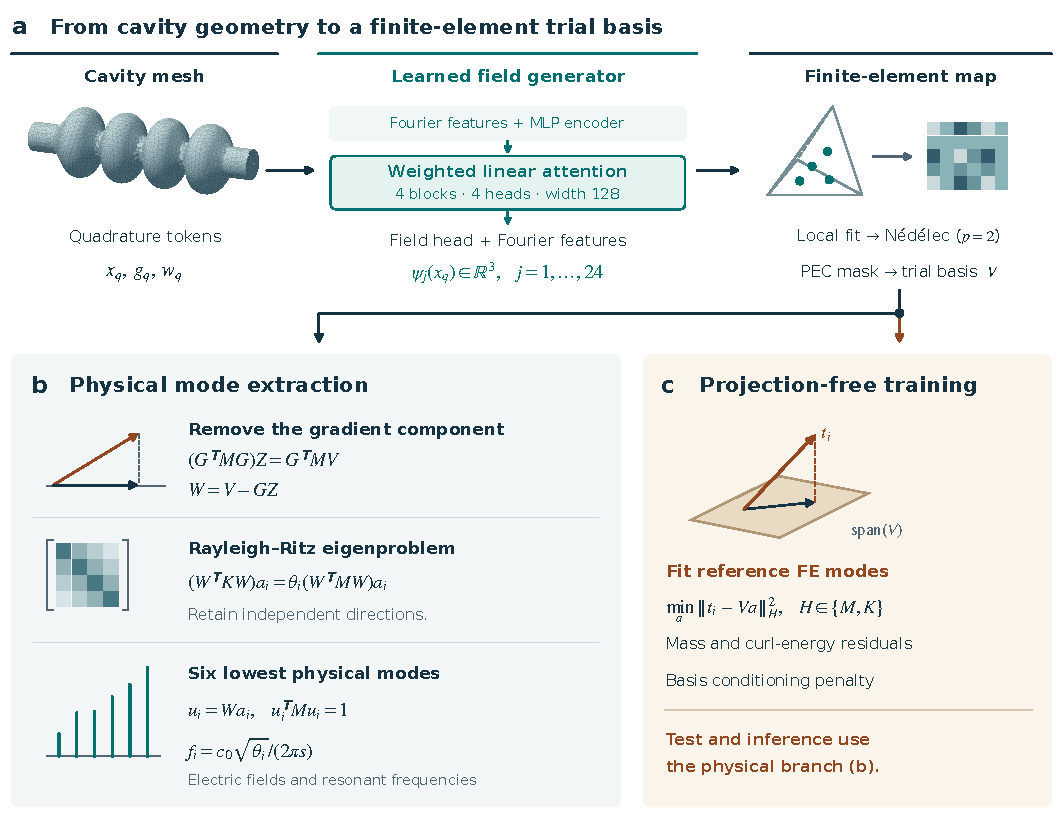
\includegraphics[width=\textwidth]{rf-model-en.pdf}
  \caption{Neural operator for resonant modes of three-dimensional RF cavities.
  (a) Each volume quadrature point supplies its position $x_q$, geometric features $g_q$, and normalized integration weight $w_q$. The weights enter the linear attention sum. The network generates 24 vector fields. An elementwise polynomial fit and interpolation into the second-order Nédélec space produce finite-element coefficients. Zeroing tangential degrees of freedom at the perfectly conducting (PEC) wall gives the trial basis $V$.
  (b) At inference, the discrete gradient $G$ and mass matrix $M$ remove the gradient component. A Rayleigh--Ritz solve with the curl--curl stiffness matrix $K$ yields electric fields and frequencies for the six lowest modes when the retained rank is sufficient. Here $c_0$ denotes the speed of light in vacuum and $s$ the length used to normalize the geometry. The spectral lines are schematic.
  (c) In the projection-free configuration shown, each reference finite-element mode $t_i$ is approximated in the span of $V$ in both the mass and curl-energy measures. Training and validation combine relative residuals with a basis-conditioning term.}
  \label{fig:rf-model-en}
\end{figure*}
